\part{Streszczenie}
Niniejszy dokument zawiera wyniki pomiaru czasu, którego potrzebował mój komputer na zapełnienie zaimplementowanych przeze mnie struktur danych: stos, kolejka oraz lista zestawami danych o długościach od 1 do 10e7 elementów. Zawiera także dokumentację kodu, który pojawił się w projekcie od poprzedniego sprawozdania.

\part{Sprawozdanie}
Obliczenia wykonano na 64-bitowym procesorze AMD Athlon X2. Wykres przedstawia zależność czasu wykonywania operacji od długości ciągu danych. Podziałki na obydwu osiach są w skali logarytmicznej. Zależności czasowe dla zapełniania stosu i kolejki są prawie identyczne i ich złożoność jest O(n); wynika to z obranego sposobu implementacji - klasy reprezentujące te struktury danych są pochodnymi pewnej klasy bazowej, po której dziedziczą metodę ładowania do struktury, a więc dla obydwu baz danych proces przebiega identycznie. Mimo to przeprowadzono badanie osobno dla każdej z tych baz danych. Gdyby badnie dotyczyło zdejmowania elementów z tych struktur danych, wyniki z pewnością różniłyby się. 

Klasa Kontener, która miała stanowić bazę do implementacji zadanych struktur przybrała w trakcie tworzenia formę listy jednokierunkowej, do której ładowanie danych okazało się ciężkim zadaniem dla komputera. Lista powinna zezwalać na dodawanie i usuwanie elementów w dowolnym miejscu i pod takim właśnie kątem została zbadana. Symulacje pokazały, że czas wykonywania operacji już dla niewielkich zestawów danych rośnie w bardzo dużym tempie. To pozostawia szerokie pole do optymalizacji programu
\centerline{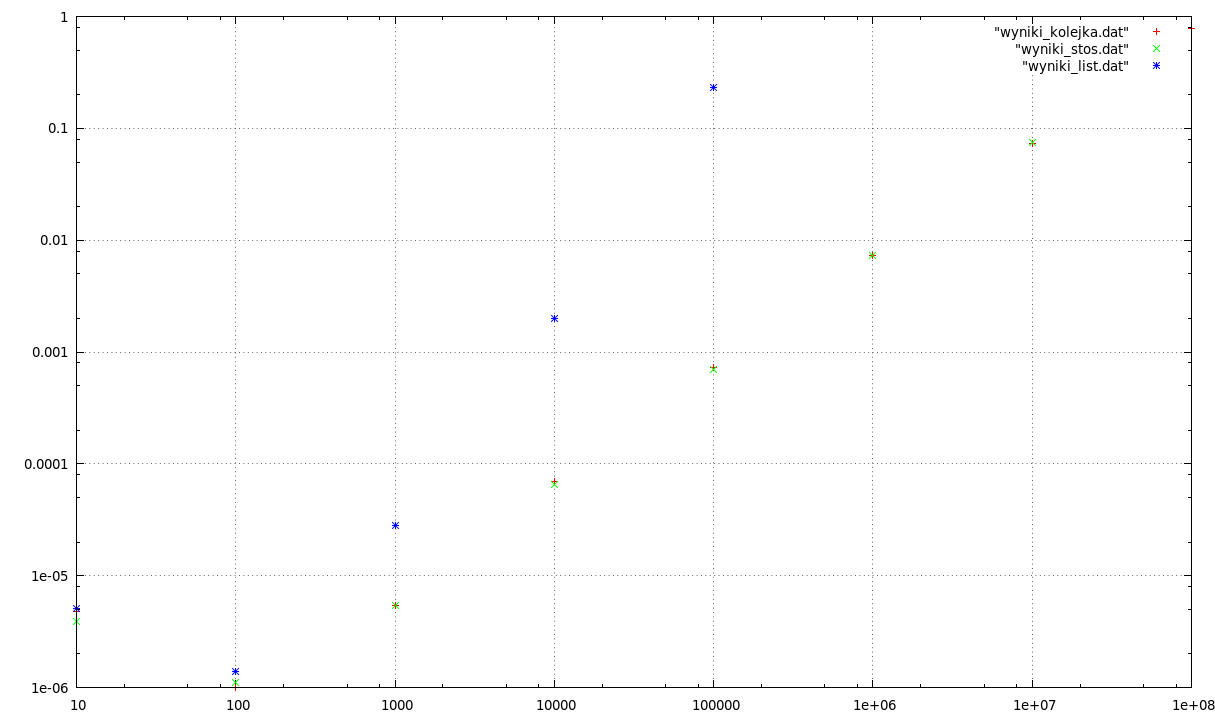
\includegraphics[width=\textwidth,height=\textheight,keepaspectratio]{wykres2.png}}
